\documentclass[a4paper,12pt]{report}
\usepackage[utf8]{inputenc}
\usepackage[dutch]{babel}
\usepackage{geometry}
\usepackage{graphicx}
\usepackage{lmodern}
\usepackage{amsmath, amssymb}
\usepackage[T1]{fontenc}
\usepackage{xcolor}
\usepackage{setspace}
\usepackage{tocbibind}
\usepackage{array} 
\usepackage{multicol}
\usepackage{tikz}
\usetikzlibrary{arrows.meta, positioning}
\usepackage[hidelinks]{hyperref}
\usepackage{titlesec} 
\usepackage{algorithm}
\usepackage{algpseudocode}


\titleformat{\chapter}[display]
  {\normalfont\huge\bfseries} % Format of chapter title
  {\centering \fontsize{120pt}{140pt} \selectfont \thechapter} % Chapter number format
  {0pt} % Space between chapter number and title
  {\vspace{0.5em}\Huge \centering} % Line between number and title, and vertical space

\titlespacing*{\chapter}{0pt}{-20pt}{20pt} % {left}{before}{after}




% \setlength{\cftbeforetoctitleskip}{-20pt} % Adjust space before ToC title
% % \setlength{\cftaftertoctitleskip}{20pt}  % Adjust space after ToC title


\setlength{\parskip}{0.8em}
\setlength{\parindent}{0pt}

\geometry{a4paper, top=3cm, bottom=3cm, left=3cm, right=3cm} 

\begin{document}

\begin{titlepage}
  \centering
  \vspace*{0cm}

  \Huge\textbf{Reinforcement Learning en Computerspellen} \\
  \vspace{1cm}
  \rule{\linewidth}{0.4mm}
  \Large
  Hoe beïnvloeden de specifieke kenmerken van computerspellen de effectiviteit van specifieke reinforcement learning-algoritmes?
  \rule{\linewidth}{0.4mm}

  \vspace{1.5cm}
  
\includegraphics[width=0.2\textwidth]{logo-clz.png} \\
  \vspace{1.5cm}
  \large
  \textbf{Matthijs Gorter} \\
  \textbf{Thom Brinkhorst} \\
  \textbf{Pepijn van Iperen} \\
  \vspace{\fill}
  \normalsize

  Profielwerkstuk \\ onder begeleiding van \\ \textit{\textbf{S. Rook}} \\
  Christelijk Lyceum Zeist \\ Natuur en Techniek \\ Februari 2025 \\ \newpage
\end{titlepage}

\chapter*{Voorwoord}
\addcontentsline{toc}{chapter}{Voorwoord} % Voeg toe aan de inhoudsopgave
Voorwoord inhoud hier. Bedank mensen die geholpen hebben, beschrijf het doel van het profielwerkstuk en eventuele persoonlijke motieven of ervaringen.

\vspace{1cm}
\noindent
Matthijs Gorter, Thom Brinkhorst, Pepijn van Iperen \\
Christelijk Lyceum Zeist \\
Februari 2025

\chapter*{Variabelen en Notatie}
\addcontentsline{toc}{chapter}{Variabelen en Notatie} % Voeg toe aan de Inhoudsopgave
\begin{table}[h]
  \begin{tabular}{>{\raggedright}p{2.5cm} >{\raggedright\arraybackslash}p{10cm}}
    \textbf{Variabele}       & \textbf{Definitie}                                \\
    \rule{\linewidth}{0.4mm} & \rule{\linewidth}{0.4mm}                          \\
    $t$                      & Tijdstap                                          \\
    $T$                      & Laatste tijdstap van een episode (horizon)        \\
    $x$                      & Toestand (state)                                  \\
    $x_t$                    & Toestand op tijdstip $t$                          \\
    $x'$                     & Toestand een tijdstap na $x$                      \\
    $\mathcal{X}$            & Set van alle toestanden                           \\
    $a$                      & Actie                                             \\
    $\mathcal{A}$            & Alle mogelijke acties                             \\
    $a_t$                    & Actie op tijdstip $t$                             \\
    $r$                      & Beloning (reward)                                 \\
    $\mathcal{R}$            & Set van mogelijke beloningen                      \\
    $r_t$                    & Beloning op tijdstip $t$                          \\
    $r(x, a)$                & Beloningsfunctie                                  \\
    $\mu$                    & Deterministisch beleid                            \\
    $\pi$                    & Stochastisch beleid                               \\
    $\pi^*$                  & Optimale stochastisch beleid                      \\
    $\gamma$                 & Kortingsfactor tussen 0 en 1                      \\
    $p(x'|x, a)$             & Overgangswaarschijnlijkheidsfunctie               \\
    $\mathcal{P}$            & Overgangswaarschijnlijkheidsmatrix                \\
    $V(x)$                   & Waardefunctie                                     \\
    $Q(x, a)$                & Q-functie                                         \\
    $Q^*(x, a)$              & Q-functie met het optimale beleid                 \\
    $\mathbb{E}[X]$          & Verwachtingswaarde van variabele $X$              \\
    $\mathbb{E}[a|b]$        & Geconditioneerde verwachtingswaarde               \\
    $\mathbb{E}_{\pi}[X]$    & Verwachtingswaarde als beleid $\pi$ wordt gevolgd \\
  \end{tabular}
  \caption{Variabelen en Notatie}
\end{table}
\newpage

\tableofcontents

\chapter{Inleiding}
Introductie Onderwerp \\ Onderwerpkeuze verantwoorden \\
Onderzoeksvraag/Hoofdvraag met eventuele hypothese \\ Deelvragen \\ Wat zijn de
specifieke kenmerken van verschillende soorten computerspellen? \\ Welke
reinforcement learning-algoritmes zijn beschikbaar en wat zijn hun kenmerken?
\\ Hoe beïnvloeden de spelkenmerken de prestatie van reinforcement
learning-algoritmes? \\ klein stukje theorie als inleiding op het
theorie-onderdeel \\ werkplan in grote lijnen, opbouw van verslag \\

\chapter{Theoretisch Kader}

\section{Definitie}
Reinforcement Learning (RL) is een tak binnen kunstmatige intelligentie waarin
een agent leert door interactie met zijn omgeving. Een agent is een entiteit
die leert en acties onderneemt. Bij een zelfrijdende auto is het
besturingssysteem de agent, en bij een schaakspel is de schaker de agent. De
omgeving is alles waarmee de agent interageert en die reageert op de acties van
de agent. Bij een zelfrijdende auto is dit de weg waar de auto op rijdt en de
voertuigen om de auto heen. Bij een schaakspel is dit het schaakbord.

De agent leert door interactie met zijn omgeving. De agent ontvangt beloningen
of straffen (negatieve beloningen) als gevolg van zijn acties. Het doel van de
agent is om een strategie te ontwikkelen die de cumulatieve beloning
maximaliseert over tijd. Bij Super Mario Bros (1985) is Mario de agent en de
agent krijgt een beloning als Mario richting de eindslag beweegt (meestal naar
rechts) en als Mario een coin of een power up oppakt en Mario krijgt een straf
als Mario sterft en hij krijgt elke seconde straf zodat hij zo snel mogelijk
het level wilt voltooien.

Figuur~\ref{fig:rl_model} illustreert het basismodel van interactie binnen
Reinforcement Learning.
\begin{figure}[h]
  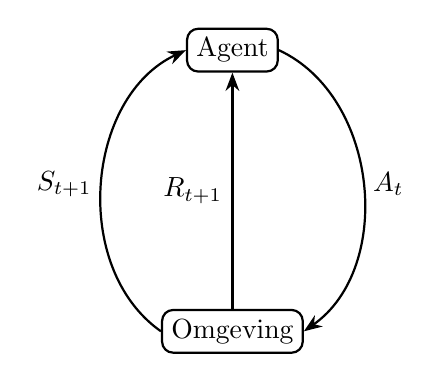
\begin{tikzpicture}[auto, thick, node distance=2cm,>=Stealth]
    \node[draw, rectangle, rounded corners] (agent) {Agent};
    \node[draw, rectangle, rounded corners, below=of agent, yshift=-1cm] (environment) {Omgeving};

    % Action arrow with adjusted bend
    \draw[->] (agent.east) to[bend left=60] node[midway, right] {$A_t$} (environment.east);

    % State arrow with adjusted text position
    \draw[->] (environment.north) to node[midway, left] {$R_{t+1}$} (agent.south);

    % Reward arrow with adjusted text position
    \draw[->] (environment.west) to[bend left=60] node[midway, left] {$S_{t+1}$} (agent.west);
  \end{tikzpicture}
  \caption{Reinforcement learning interactiemodel tussen agent en omgeving via acties, toestanden en beloningen.}
  \label{fig:rl_model}
\end{figure}

Een actie naar de beslissing die een agent neemt bij elke stap in een
besluitvormingsproces. Acties worden aangeduid met \( a \) en worden gekozen
uit een reeks mogelijke acties \( \mathcal{A} \). Elke door de agent genomen
actie beïnvloedt de interactie met de omgeving, wat leidt tot een verandering
in de toestand en een daaruit voortvloeiende beloning.

Een toestand \( x \) vertegenwoordigt de huidige situatie of staat van de
omgeving waarin de agent opereert. Dit wordt aangeduid met \( x \) en maakt
deel uit van de toestandsruimte \( \mathcal{X} \). Bij de aanvangsstap \( t = 0
\), begint de agent in een initiële toestand \( x_0 \) die willekeurig wordt
bepaald door een verdeling \( p \). Naarmate het proces vordert, bevindt de
agent zich in nieuwe toestanden gebaseerd op zijn acties.

Een beloning \( r \) is een feedbackwaarde die wordt ontvangen nadat de agent
een actie heeft uitgevoerd in een bepaalde toestand. Deze beloning wordt
bepaald door de beloningsfunctie \( r(x, a) \). De beloningsmatrix \( R \)
bevat de onmiddellijke beloningen voor elke combinatie van toestand en actie.

Een overgang beschrijft de verandering van de huidige toestand naar de volgende
toestand als gevolg van een actie die door de agent wordt genomen. De
waarschijnlijkheid van overgang wordt bepaald door de
overgangswaarschijnlijkheidsfunctie \( p(x'|x, a) \), die afhangt van de
huidige toestand \( x \), de genomen actie \( a \) en leidt tot een nieuwe
toestand \( x' \). De overgangswaarschijnlijkheidsmatrix \( P \) bevat de
waarschijnlijkheden van het overgaan van de ene toestand naar de volgende
toestand, gegeven een bepaalde actie.

\section{Belangrijke Algoritmes}

\begin{algorithm}
  \caption{Example Algorithm}
  \begin{algorithmic}[1] % The number 1 means line numbers will start at 1
      \State \textbf{Input:} An array $A$ of $n$ integers
      \State \textbf{Output:} The sum of the integers in $A$
      \State $sum \gets 0$
      \For{$i \gets 1$ to $n$}
          \State $sum \gets sum + A[i]$
      \EndFor
      \State \Return $sum$
  \end{algorithmic}
  \end{algorithm}

\section{Artificiële Leermethodes}

\section{Computerspellen}

\chapter{Onderzoeksmethoden}

\chapter{Analyse en Resultaten}

\chapter{Conclusie}

\chapter{Discussie}

\chapter{Referentielijst}

\chapter{Bijlagen}

\end{document}
